\documentclass{article}

\oddsidemargin=0in
\evensidemargin=0in
\textwidth=6in
\topmargin=0in
\textheight=9in

\parindent=0in
\pagestyle{empty}

\usepackage{amsfonts}
\usepackage{amssymb}
\usepackage[pdftex]{graphicx}
\usepackage{multirow}

\begin{document}

\section*{Chapter 1:  Explanation of the Algorithm} 
 \noindent The problem which needs to be solved is as follows: there are a number of objects, which all have a size and a value, and we have a knapsack which has a capacity. This means that it only can take a certain amount of objects. These objects should amount to a value that is as large as possible.\\

\begin{figure}[h!]
  \centering
      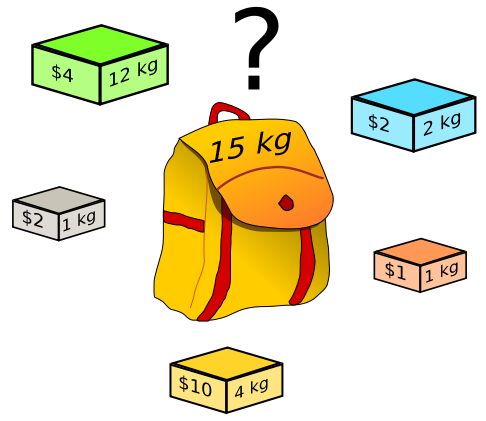
\includegraphics[width=0.5\textwidth]{Knapsack.png}
  \caption{An illustration of the Knapsack problem! \textbf{ADD REF HERE} }
\end{figure}

\textbf{Elementary operation:} We are counting the number of objects that are in the input file defined as n, and the number of possible subsets which can be created from them ($2^n$), defined as m.\\

\noindent \textbf{Pseudocode:}
\begin{tabbing}
For \= all the objects in the input file \\
\> create \= all possible subsets	\\
\> select the best subset with the highest value\\
\end{tabbing}

After reading the input file and putting each of these objects into a Tuple which has a size and a value, the Algorithm exists of two parts. First of all, the algorithm creates all possible subsets of the input Tuples, and second of all it selects the first subset which has a size less or equal to the capacity of the knapsack and has the highest value.\\
 

\section*{Chapter 2: Algorithm in Pseudocode}
In this chapter the algorithm will be explained in more detail. The following is the pseudocode for the function "createPowerset()". \newline

\begin{verbatim}
n = Size of the tuple list 	
m = Size of possible subsets 2^n

for i = 0 to  m-1 loop
  element = 1  
  create temporary arraylist  
    for j = 0 to n-1 loop
       if (i "bitwise and" element is not 0)
         add tuple to temporary arraylist
       end if
       element = element << 1
    end for
    add subset to list
end for
 
\end{verbatim}

\noindent This function creates a power set[reference], which is a set of all possible subsets of the set. It is known that the power set will have $2^n$ subsets. Through bit masking with the bitwise "and" operator and letting i = 1 to m represent all possible subsets, it is checked if the corresponding bits are both 1, in which case the current tuple is saved in a temporary array list. Using the shift left operator $<<$ the element is shifted one step to the left before next iteration to enable checking if the next element is part of the current subset. The final step before next iteration is to add the resulting subset to the list of subsets. \\ \\ 

The second part of the algorithm is to select the best possible subset and is shown in the pseudocode below.\\

\begin{verbatim}
k = Size of list containing all possible subsets
capacity = the capacity of the knapsack
bestValue = the best value of all subsets (intiated to 0)
bestSet = the set that gives bestValue

for i = 1 to k loop

  sumSizes = 0
  sumValue = 0

  for j = 1 to size of subset i loop
    tuple = tuple j from subset i
    add the size of the tuple to sumSizes and store in sumSizes
    add the value of the tuple to sumValue and store in sumValue
  end for

  if (sumSizes is less than or equal to the capacity)
    if(sumValue is greater than bestValue)
      store sumValue as bestValue
      store set i as bestSet
    end if
  end if
end for
\end{verbatim}

\noindent This part of the algorithm is a greedy algorithm which chooses the best possible subset for the Knapsack problem, if several subsets produces equally good value the first such subset is selected. The function loops through all created subsets and adds up all sizes and values of the tuples in that subset. It then checks if the sum of the sizes is less than or equal to the capacity of the Knapsack and if it is it will check if the sum of the values of this subset is better than the previous bestValue. If a new bestValue was optained it will be stored as bestValue and also the subset giving this bestValue will be stored until the algorithm finds a subset which results in a better value.\\

\section*{Chapter 3: Correctness Justification}

\section*{Chapter 4: Complexity Analysis}

\section*{Chapter 5: Performance Test}

The time for each test is measured in milliseconds. The tests were done by using java.lang.System.currentTimeMillis() to get one start time as the first thing done in the createPowerset method in the algorithm, and one stop time at the second last line (before calling the printBestSet method) in selectBestSet. The resulting execution time was calculated by subtrackting the the start time from the stop time to get a result of how long the algorithm was executing with the different input files.\\

\begin{tabular}{|l|l|l|} \hline
Items &Capacity &Execution time\\ \hline
\multirow{3}{*}{10} & 6 & 11 \\
& 20 & 11 \\
& 35 & 10 \\ \hline
\multirow{3}{*}{15} & 6 & 57 \\
& 20 & 61 \\
& 35 & 59 \\ \hline
\multirow{3}{*}{20} & 6 & 1460 \\
& 20 & 1447 \\
& 35 & 1445 \\ \hline
\end{tabular}

\section*{Appendix 1: Compile and run program}
\noindent Compile the program with 'javac Knapsack.java'\\ 
\noindent Run the compiled program with 'java Knapsack ``inputfile.txt''' where inputfile is the name of the input file. If no input file is provided, the instance 3 input file given in the problem is used as default. 

\section*{Appendix 2: References}
%Add referens for wiki pic

%add ref for the idea to use bitmasking http://www.mathsisfun.com/sets/power-set.html


\end{document}
